\section*{The Probabilistic Framework}
Our solution is based on discrete \emph{Markov processes}, which are a special case of stochastic processes. For a Markov process, the next state depends only on the present state and not on past states.

An example of a discrete Markov process is that of throwing dice and summing the results: the throws and state space are discrete, and the possible states (sums) after the next throw depend only on the current state.

In mathematical terms, a discrete Markov process satisfies the following:
\begin{equation}
 \cprob{Z_{n+1}}{Z_n \wedge Z_{n-1} \wedge \dots \wedge Z_0} = \cprob{Z_{n+1}}{Z_n}
\end{equation}
where $Z_n$ is the system's \emph{state} after step $n$ and $\cprob{Z_{n+1}}{Z_n \wedge Z_{n-1} \wedge \dots \wedge Z_0}$ is the probability that the system will have state $Z_{n+1}$ in the next step, given that the previous states were $Z_n, Z_{n-1}, Z_{n-2}, \dots, Z_0$.

A \emph{hidden Markov model} (HMM) describes a Markov process where one cannot measure the state $Z$ of the system directly - it is ``hidden'' - but rather obtains an \emph{observation} $I$\footnote{In this project, the observation is a grayscale \emph{image}, which is why we use the symbol $I$.}  of the state by some \emph{perception}. The observation is generally non-deterministic, so we need to denote it as $p(I_n|Z_n)$ which is the probability that we will observe $I_n$ if the current state of the system is $Z_n$.

\subsection*{The Particle Filter}
The Particle Filter is a technique for simulating a process described by a HMM. It uses a finite set $X_n$ of $N$ hypotheses to approximate the probability function $p(Z_n)$ above. The hypotheses $X_n$ are also known as \emph{particles}, thereby the term ``particle filter''. In short terms, the particle filter does the following:

\begin{enumerate}
  \item Predicts the next state $Z_{n+1}$ by drawing samples $X_{n+1}$ from $p(Z_{n+1} | Z_n)$,
  \item resamples the hypotheses $X_{n+1}$ by drawing new samples from $p\left(I_{n+1} | x_{n+1}^i\right)$
\end{enumerate}


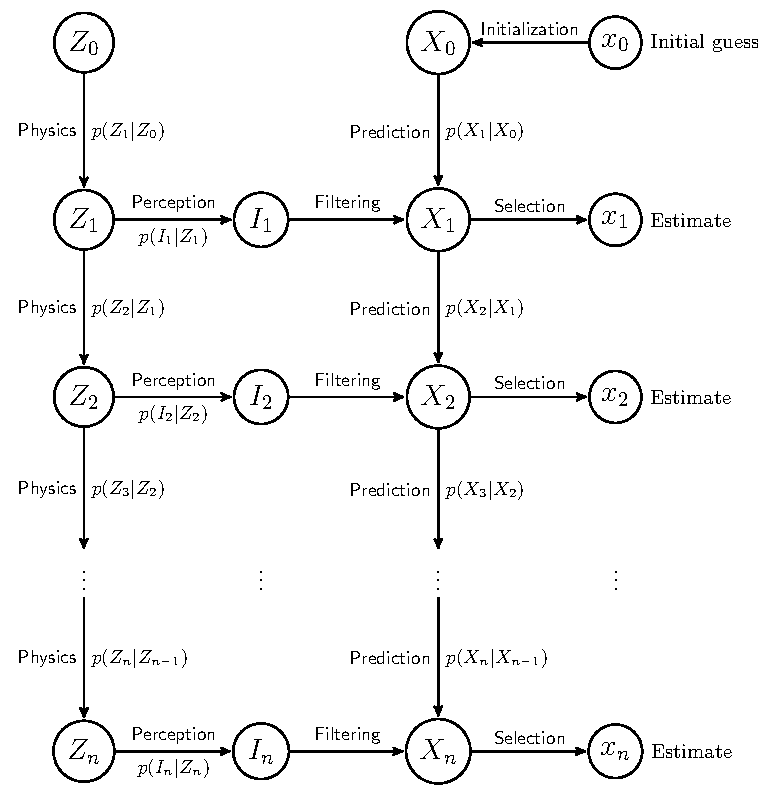
\includegraphics[width=0.3\textwidth]{figures/hmm-graph/hmm-graph.pdf}
Above is an illustration of a Particle Filter working with a Hidden Markov Model. The system assumes states $Z_0, Z_1, ...$ with probabilities $p(Z_0), p(Z_1|Z_0), \cdots$, and we obtain the observations $I_1, I_2, \cdots$ with probabilities $p(I_1|Z_1), p(I_2|Z_2), \cdots$. Parallel to this, we have a set of hypotheses $X$ for the state $Z$. The hypotheses $X_n$ of $Z_n$ are updated in the \emph{prediction} step to hypotheses $\bar{X}_{n+1}$ of $Z_{n+1}$. The image $I_{n+1}$ of the system is then used in the \emph{resampling step} to select the best hypotheses from $\bar{X}_{n+1}$, yielding the \emph{belief} $X_{n+1}$. Finally, we create a single hypothesis $x_{n+1}$ from $X_{n+1}$ that will be our estimate of the state $Z_{n+1}$.
